%!TEX TS-program = xelatex
\documentclass{EdipyLabs} % Custom class provided for EDIPY labs, by Christos Dalamagkas (cdalamagkas@gmail.com)
\SetLabNumber{3}
\SetLabTitle{Υποδικτύωση IPv4}
\SetAuthor{Χρήστος Δαλαμάγκας}
\SetLabDescription{Υποδικτύωση IPV4, τεχνικές FLSM και VLSM, μήκος προθέματος, μάσκα υποδικτύου, CIDR.}
\SetLabPrerequisites{Εργαστηριακό φυλλάδιο 2α (Διευθέτηση δρομολογητή), Βασικές γνώσεις υποδικτύωσης και διευθυνσιοδότησης IPv4.}

\usepackage{pdflscape}
\usepackage{afterpage}

\begin{document}
\Initialize

\section*{Εισαγωγή}
Η υποδικτύωση αποτελεί μια από τις σημαντικότερες εργασίες ενός διαχειριστή δικτύου, η υλοποίηση της οποίας προσφέρει πολλαπλά οφέλη. Συνοπτικά, μέσω της υποδικτύωσης μπορεί κάποιος να αυξήσει τη συνολική δικτυακή απόδοση, περιορίζοντας την έκταση του τομέα ευρυεκπομπής (broadcast domain)\footnote{Ακριβέστερα, για τον περιορισμό του τομέα ευρυεκπομπής η υποδικτύωση συνδυάζεται με VLAN, τα οποία εξετάζονται σε επόμενο εργαστηριακό φυλλάδιο.}, να εφαρμόσει πολιτικές ασφαλείας αλλά και να οργανώσει καλύτερα ένα μεγάλο δίκτυο. 

Στο παρόν εργαστηριακό φυλλάδιο θα υλοποιήσετε δυο σενάρια υποδικτύωσης, με το πρώτο να αφορά υποδίκτυα ίδιου μεγέθους (Fixed Length Subnet Masking - FLSM) και το δεύτερο διαφορετικού μεγέθους (Variable Length Subnet Masking - VLSM). Αν και η υποδικτύωση είναι γνωστή από το μάθημα «Δίκτυα Υπολογιστών Ι/ΙΙ», στο φυλλάδιο συμπεριλαμβάνεται μια συνοπτική παράθεση του απαραίτητου θεωρητικού υποβάθρου, με έμφαση σε τεχνικές που επιτρέπουν τους γρήγορους αριθμητικούς υπολογισμούς. 

\begin{warningblock}
	Προτείνεται να \textbf{μην χρησιμοποιείτε} ηλεκτρονικές συσκευές για την εκτέλεση αριθμητικών πράξεων. Απαιτείται από τους μηχανικούς δικτύων η μέγιστη δυνατή εξοικείωση με τον χειρισμό διευθύνσεων IP, ώστε οι ίδιοι να είναι σε θέση να εργάζονται αυτοματοποιημένα, εντοπίζοντας και διορθώνοντας γρήγορα και αποτελεσματικά προβλήματα στα δίκτυα IP.
\end{warningblock}

Για την υλοποίηση της τοπολογίας θα χρειαστείτε τις εξής συσκευές:
\begin{itemize}
	\item x2 δρομολογητές Cisco 2921
	\item x2 μεταγωγείς Catalyst 2960-SF 
\end{itemize}

\section*{Παραδοτέα}
\begin{itemize}
	\item Tο παρόν PDF με συμπληρωμένα \textbf{όλα} τα πεδία.
	\item Με την ολοκλήρωση των σεναρίων Α και Β:
	\begin{itemize}
		\item Αρχείο με τις τρέχουσες ρυθμίσεις του δρομολογητή R1.
		\item Αρχείο με τις τρέχουσες ρυθμίσεις του δρομολογητή R2.
		\item Στιγμιότυπο οθόνης που δείχνει επιτυχημένη εκτέλεση του traceroute από το PC1 προς το PC2.
	\end{itemize}
\end{itemize}
\newpage

\begin{figure}
	\centering
	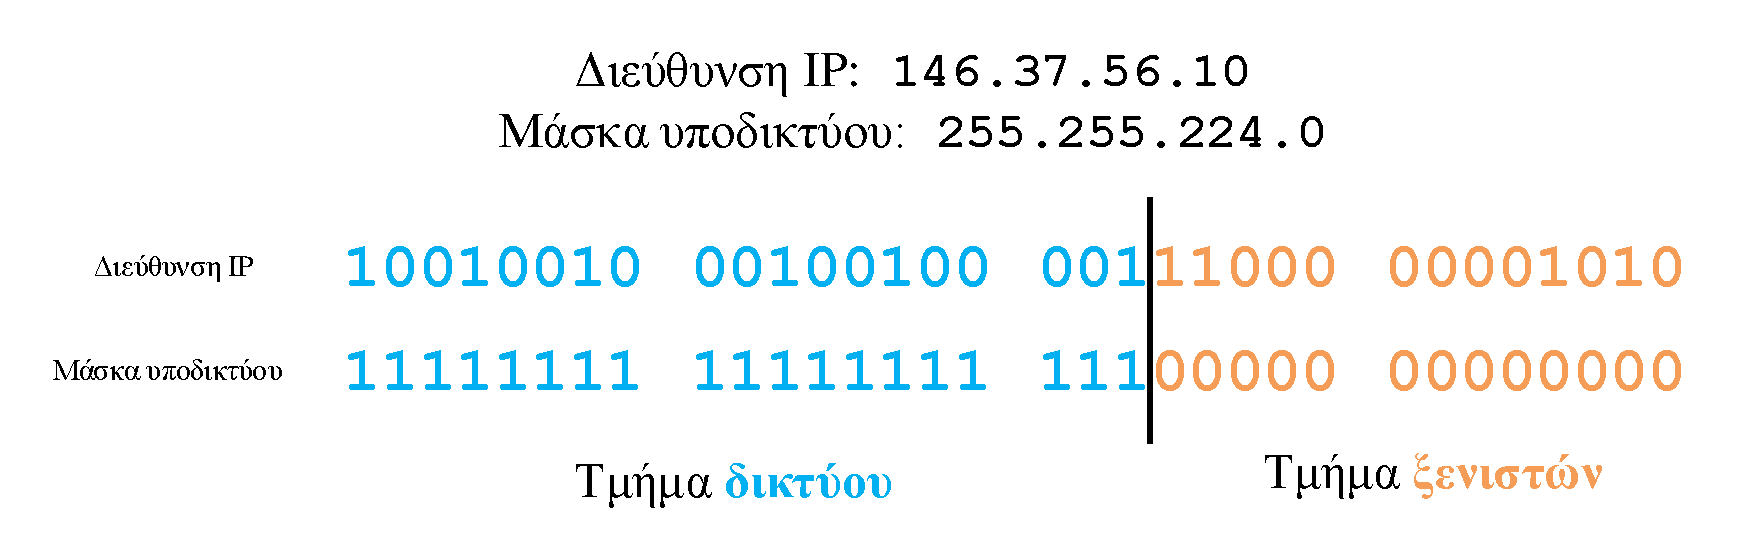
\includegraphics[width=\linewidth]{ip}
	\caption{Πως η μάσκα δικτύου διαχωρίζει τα τμήματα μιας διεύθυνσης IP}\label{fig:ip}
\end{figure}

\section{Θεωρητικό υπόβαθρο}
Μια διεύθυνση IP είναι ένας αριθμός μεγέθους 32 bit, στο δυαδικό σύστημα, ο οποίος χρησιμοποιείται για την αναγνώριση μιας δικτυακής οντότητας σε ένα δίκτυο. Η διεύθυνση IPv4 αποτελείται από το τμήμα δικτύου και το τμήμα ξενιστών\footnote{«Ξενιστής» ορίζεται οποιαδήποτε δικτυακή συσκευή φιλοξενείται σε ένα δίκτυο: υπολογιστής, δρομολογητής, μεταγωγέας.}, όπως φαίνεται στο σχήμα \ref{fig:ip}. Το \textbf{τμήμα δικτύου} (network portion) δείχνει σε ποιο δίκτυο ανήκει μια δικτυακή συσκευή, ενώ το \textbf{τμήμα ξενιστών} (host portion) ορίζει το αναγνωριστικό της μέσα στο δίκτυο. Αναλογικά, θα μπορούσαμε να αντιστοιχίσουμε το τμήμα δικτύου με το επώνυμο ενός ανθρώπου και το τμήμα ξενιστών με το μικρό του όνομα. Το επώνυμο δηλώνει την οικογένεια (δίκτυο IP), στην οποία ανήκει ο άνθρωπος, και το μικρό όνομα (τμήμα ξενιστών) συμπληρώνει το πλήρες ονοματεπώνυμο (διεύθυνση IP) κάποιου.

\begin{table}[ht!]\centering\renewcommand{\arraystretch}{1.5}\rowcolors{1}{lightgray}{white}
	\begin{tabular}{llll}
		\FormatFirstRow
		\textbf{Πρώτη διεύθυνση} & \textbf{Τελευταία διεύθυνση} & \textbf{Κλάση} & \textbf{Μάσκα υποδικτύου} \\
		0.0.0.0			& 127.255.255.255	  & A	  & 255.0.0.0		  \\
		128.0.0.0		& 191.255.255.255	  & B	  & 255.255.0.0		  \\
		192.0.0.0		& 223.255.255.255	  & C	  & 255.255.255.0
	\end{tabular}
	\caption{Οι τρείς βασικές κλάσεις διευθυνσιοδότησης.}\label{tab:clasful}
\end{table}

Το μέγεθος του τμήματος δικτύου καθορίζεται από τη \textbf{μάσκα υποδικτύου} (subnet mask). Η μάσκα υποδικτύου είναι ένας αριθμός 32 bit, ο οποίος λαμβάνει τιμή 1 στις θέσεις της διεύθυνσης IP που αντιστοιχούν στο τμήμα δικτύου και 0 στις θέσεις που αντιστοιχούν στο τμήμα ξενιστών. Παράδειγμα εφαρμογής της μάσκας υποδικτύου απεικονίζεται στο σχήμα \ref{fig:ip}, όπου φαίνεται το πως η μάσκα υποδικτύου διαχωρίζει το τμήμα δικτύου από το τμήμα ξενιστών. Εφαρμόζοντας την πράξη AND μεταξύ της μάσκας και μιας διεύθυνσης IP προκύπτει η \textbf{διεύθυνση δικτύου} (network address) ή \textbf{πρόθεμα δικτύου} (network prefix).

Όταν αναφερόμαστε σε ταξική διευθυνσιοδότηση (classful addressing), το μέγεθος του τμήματος δικτύου, δηλαδή η μάσκα υποδικτύου, είναι εκ των προτέρων γνωστή, παρατηρώντας σε πιο εύρος ανήκει η διεύθυνση δικτύου. Στον πίνακα \ref{tab:clasful} παρατίθενται οι τρεις κύριες κλάσεις διευθύνσεων. Ωστόσο, τα σύγχρονα δίκτυα και πρωτόκολλα δεν χρησιμοποιούν πια τις κλάσεις για να προσδιορίσουν τη μάσκα υποδικτύου. Πλέον η ταξική διευθυνσιοδότηση έχε αντικατασταθεί από την μέθοδο Αταξικής Δρομολόγησης Δικτυακών Περιοχών (Classless Inter-Domain Routing - CIDR). Η εν λόγω μέθοδος επιτρέπει τον ορισμό οποιουδήποτε μεγέθους τμήματος δικτύου για μια διεύθυνση IP, αρκεί αυτή να συνοδεύεται από τη μάσκα υποδικτύου.

Η μάσκα υποδικτύου μπορεί να αξιοποιηθεί για διάφορους υπολογισμούς. Στον πίνακα \ref{tab:trics} συνοψίζονται όλοι οι δυνατοί υπολογισμοί για μια διεύθυνση IP, αξιοποιώντας παράλληλα τη μάσκα υποδικτύου.

\begin{assignmentbox}
	Με βάση τις μεθόδους του πίνακα \ref{tab:trics}, υπολογίστε τα πεδία του πίνακα \ref{tab:askisi} για τη διεύθυνση \textbf{\texttt{143.65.21.4/20}}.
\end{assignmentbox}

\begin{table}\centering
	\begin{MyTabularAuto}{Στοιχείο}{Τιμή}
		Μάσκα υποδικτύου σε δυαδική μορφή 		& \textField{1}{4cm}{0.5cm} \\
		Μάσκα υποδικτύου σε δεκαδική μορφή 		& \textField{2}{4cm}{0.5cm} \\
		Διεύθυνση δικτύου 						& \textField{3}{4cm}{0.5cm} \\
		Διεύθυνση ευρυεκπομπής 					& \textField{4}{4cm}{0.5cm} \\
		Πρώτη ωφέλιμη διεύθυνση 				& \textField{5}{4cm}{0.5cm} \\
		Τελευταία ωφέλιμη διεύθυνση 			& \textField{6}{4cm}{0.5cm} \\
		Μέγεθος δικτύου σε ωφέλιμες διευθύνσεις & \textField{7}{4cm}{0.5cm}
	\end{MyTabularAuto}
	\caption{Υπολογισμοί για τη διεύθυνση \texttt{143.65.21.4/20}}\label{tab:askisi}
\end{table}

\begin{table}\centering\renewcommand{\arraystretch}{1.5}
\begin{tabular}{ll}
	\FormatFirstRow
	\textbf{Πρόβλημα} & \textbf{Διαδικασία υπολογισμού}\\
	Μάσκα αναπλήρωσης (wildcard mask)			& Λογικό NOT στη μάσκα υποδικτύου.\\
	
	\rowcolor{lightgray}						& Λογικό AND της μάσκας υποδικτύου με τη διεύθυνση IP ή\\
	\rowcolor{lightgray}
	\multirow{-2}{*}{Διεύθυνση δικτύου} 		& Από διεύθυνση IP: 0 σε όλο το τμήμα ξενιστών. \\ 
												& Λογικό OR της μάσκας αναπλήρωσης με τη διεύθυνση IP ή\\
	\multirow{-2}{*}{Διεύθυνση ευρυεκπομπής}	& Από διεύθυνση IP: 1 σε όλο το τμήμα ξενιστών.\\
	\rowcolor{lightgray}
	Πρώτη ωφέλιμη διεύθυνση IP 					& +1 bit στη διεύθυνση δικτύου.\\
	Τελευταία ωφέλιμη διεύθυνση IP 				& -1 bit από τη διεύθυνση ευρυεκπομπής.\\
	\rowcolor{lightgray}
	Μήκος προθέματος δικτύου					& Πλήθος των 1 στη μάσκα υποδικτύου, δηλαδή 255.255.255.0 = /24.\\
	Πλήθος ξενιστών ενός δικτύου 				& $2^{h}-2$, όπου $h$ το πλήθος bit του τμήματος ξενιστών.\\
\end{tabular}\caption{Χρήσιμοι υπολογισμοί με τις μάσκες υποδικτύου/αναπλήρωσης.}\label{tab:trics}
\end{table}

\subsection{Η μέθοδος FLSM}

\begin{figure}
	\centering
	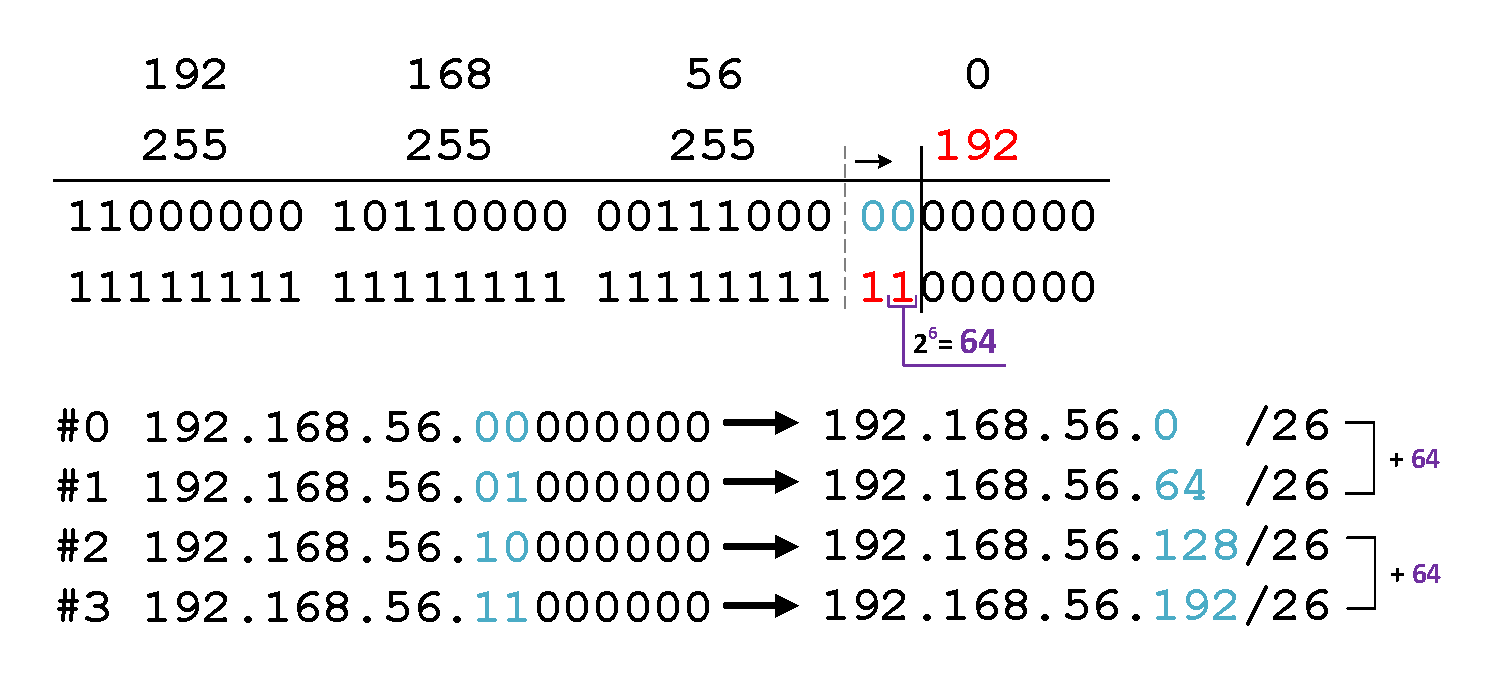
\includegraphics[width=\linewidth]{flsm}
	\caption{Παράδειγμα χωρισμού του \texttt{192.168.56.0/24} σε 4 υποδίκτυα}\label{fig:flsm}
\end{figure}

Η υποδικτύωση είναι μια διαδικασία που επιτρέπει τον χωρισμό ενός μεγάλου δικτύου, ή τομέα ευρυεκπομπής, σε μικρότερα τμήματα, τροποποιώντας την μάσκα υποδικτύου. Η πιο απλή τεχνική αφορά τον χωρισμό ενός τομέα ευρυεκπομπής σε μικρότερα, ίσα μεταξύ τους τμήματα. Η υποδικτύωση γίνεται εφικτή επεκτείνοντας το μέγεθος του τμήματος δικτύου, «δανειζόμενοι» bit από το τμήμα ξενιστών. Μεγαλύτερο τμήμα δικτύου μας επιτρέπει να ορίσουμε περισσότερα δίκτυα, με λιγότερους ξενιστές. Ένα παράδειγμα FLSM φαίνεται στο σχήμα \ref{fig:flsm}, στο οποίο χωρίζεται το \textbf{\texttt{192.168.56.0/24}} σε 4 υποδίκτυα. Για να δημιουργηθούν 4 υποδίκτυα χρειάστηκε να δανειστούμε 2 bit, αφού $2^2=4$. Με κόκκινο έχει επισυναπτεί η νέα μάσκα, η οποία έγινε \texttt{255.255.255.192} ή \texttt{/26}. Τα νέα bit από το τμήμα ξενιστών (μπλε χρώμα) διαμορφώνουν τις νέες διευθύνσεις δικτύων οι οποίες έχουν παρατεθεί στο ίδιο σχήμα.

Είναι εμφανές ότι η παραπάνω διαδικασία δε θα μπορούσε να εφαρμοστεί εύκολα για μεγαλύτερο πλήθος υποδικτύων, παραδείγματος χάριν, για τον χωρισμό ενός \texttt{/8} δικτύου σε χιλιάδες τμήματα. Μία παρατήρηση που θα μπορούσε να επιταχύνει τη διαδικασία υποδικτύωσης είναι ο λεγόμενος «\textit{\textbf{μαγικός αριθμός}}», η τιμή του οποίου υπολογίζεται από τη θέση του τελευταίου ψηφίου της μάσκας, σε σχέση με την οκτάδα στην οποία αυτό ανήκει. Για παράδειγμα, στο σχήμα \ref{fig:flsm} o μαγικός αριθμός είναι \textbf{64}, αφού το τελευταίο ψηφίο της μάσκας βρίσκεται στη θέση 6 της τελευταίας οκτάδας. 

Η τιμή του μαγικού αριθμού δείχνει το βήμα αύξησης της διεύθυνσης δικτύου στο δεκαδικό σύστημα. Ακόμη, η θέση του τελευταίου ψηφίου της μάσκας μας δείχνει ποια οκτάδα είναι αυτή στην οποία θα προστίθεται ο μαγικός αριθμός σε κάθε βήμα. Όπως φαίνεται και στο παράδειγμα του σχήματος \ref{fig:flsm}, η τελευταία οκτάδα αυξάνεται κατά 64, αφού ο μαγικός αριθμός είναι 64 και η τιμή του βρίσκεται στην τελευταία οκτάδα.

\textit{\textbf{Παράδειγμα}}: Έστω το δίκτυο \textbf{\texttt{10.0.0.0/8}}, το οποίο θέλουμε να διασπάσουμε σε τουλάχιστον 1000 υποδίκτυα: Για να αναπαραστήσουμε τουλάχιστον 1000 υποδίκτυα χρειάζεται να δανειστούμε το λιγότερο 10 bit από το τμήμα ξενιστών (αφού $2^{10}=1024$), άρα το νέο μήκος προθέματος είναι \texttt{/8 + 10 = /18}. Αναπαριστώντας το \texttt{/18} στο δυαδικό βλέπουμε ότι το τελευταίο bit της μάσκας βρίσκεται στην $6^\text{η}$ θέση της τρίτης οκτέτας. Αφού $2^6=64$, o μαγικός αριθμός είναι \textbf{64} και η διεύθυνση δικτύου θα αυξάνεται κατά $64$ στην τρίτη οκτέτα. Συνεπώς, τα υποδίκτυα διαμορφώνονται ως εξής: \texttt{10.\textbf{0.0}.0/18, 10.\textbf{0.64}.0/18, 10.\textbf{0.128}.0/18, 10.\textbf{0.192}.0/18, 10.\textbf{1.0}/18, ...,10.\textbf{255.192}.0/18}.

\subsection{Η μέθοδος VLSM}

Η μέθοδος FLSM χωρίζει ένα δίκτυο σε ίσα τμήματα, κάτι το οποίο δεν είναι πάντα πρακτικό. Για παράδειγμα, ένα δικτυακό περιβάλλον, είτε τοπικό (LAN) είτε ευρείας περιοχής (WAN), μπορεί να έχει υποδίκτυα με διαφορετικές ανάγκες, καθώς και δίκτυα σημείου προς σημείο, τα οποία χρειάζονται μήκος προθέματος \texttt{/30}. Η μέθοδος VLSM, ουσιαστικά, επιτρέπει την πολλαπλή υποδικτύωση FLSM των δικτύων με διαφορετικό μήκος προθέματος σε κάθε απόπειρα υποδικτύωσης.

Στο σχήμα \ref{fig:vlsm} παρατίθεται ένα παράδειγμα υποδικτύωσης VLSM του \textbf{\texttt{192.168.56.0/24}} σε 1 υποδίκτυο των 126 ξενιστών, 3 υποδίκτυα των 30 ξενιστών και 2 υποδίκτυα σημείου προς σημείο, των 2 ξενιστών. Δεδομένου ότι το μεγαλύτερο δίκτυο που θέλουμε είναι το \texttt{/25}, χωρίζουμε πρώτα το \texttt{/24} σε δυο υποδίκτυα των \texttt{/25} με τη γνωστή, πλέον, διαδικασία FLSM. Συνεπώς, τα νέα υποδίκτυα είναι:
\begin{itemize}
	\item \texttt{192.168.56.0/25 <-- \#0}
	\item \texttt{192.168.56.128/25}
\end{itemize}
Κρατάμε το πρώτο δίκτυο \texttt{192.168.56.0/25} ως το πρώτο από τα ζητούμενα. Στη συνέχεια, θέλουμε 3 δίκτυα των 30 ξενιστών, συνεπώς, υποδικτυώνουμε το δεύτερο τμήμα της πρώτης υποδικτύωσης, το 192.168.56.128/25 με τη μέθοδο FLSM. Ωστόσο, αυτή τη φορά θα χωρίσουμε το δίκτυο σε τμήματα νέου μήκους προθέματος \texttt{/27}:
\begin{itemize}
	\item \texttt{192.168.56.128/27 <-- \#1}
	\item \texttt{192.168.56.160/27 <-- \#2}
	\item \texttt{192.168.56.192/27 <-- \#3}
	\item \texttt{192.168.56.224/27}
\end{itemize}

Κρατάμε τα τρία πρώτα υποδίκτυα ως τα ζητούμενα δίκτυα μεγέθους \texttt{/27}. Τέλος, χρειαζόμαστε ακόμα δυο υποδίκτυα των \texttt{/30}, συνεπώς, υποδικτυώνουμε κατάλληλα το \texttt{192.168.56.224/27} που έμεινε αδιάθετο. Από τα προκύπτοντα υποδίκτυα κρατάμε μόνο τα πρώτα δυο, με τα υπόλοιπα να είναι διευθύνσεις IP που εξοικονομήσαμε με την τεχνική VLSM:
\begin{itemize}
	\item \texttt{192.168.56.224/30 <-- \#4}
	\item \texttt{192.168.56.228/30 <-- \#5}
	\item \texttt{192.168.56.232/30}
\end{itemize}

\afterpage{
\newgeometry{margin=1cm}	
\begin{landscape}
	\thispagestyle{empty} %% Remove header and footer.
	\begin{figure}
		\centering 
		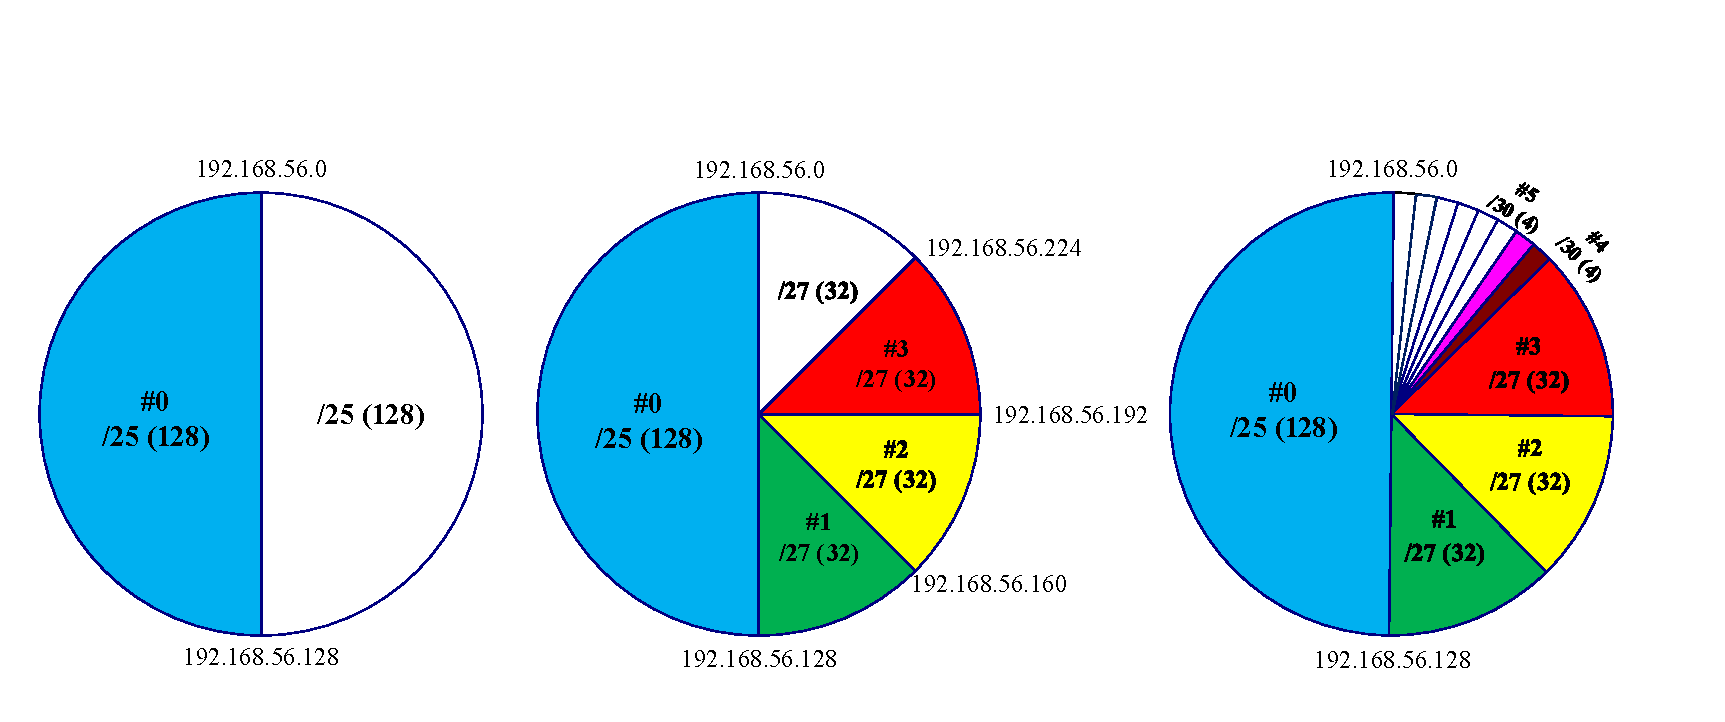
\includegraphics[trim={0.65cm 0 1.8cm 2.6cm}, clip, width=\linewidth]{vlsm}
		\caption{Γραφική αναπαράσταση της τεχνικής VLSM.}\label{fig:vlsm}
	\end{figure} 
\end{landscape}
\clearpage
\restoregeometry
}
\newpage
\restoregeometry

\section{Σενάριο: Υποδικτύωση FLSM}

H τοπολογία που θα υλοποιήσετε για το πρώτο σενάριο της εργαστηριακής άσκησης απεικονίζεται στο σχήμα \ref{fig:topology}. Ξεκινώντας, υλοποιήστε την καλωδίωση, σύμφωνα με το σχήμα της τοπολογίας.

\begin{figure}[ht]
	\centering
	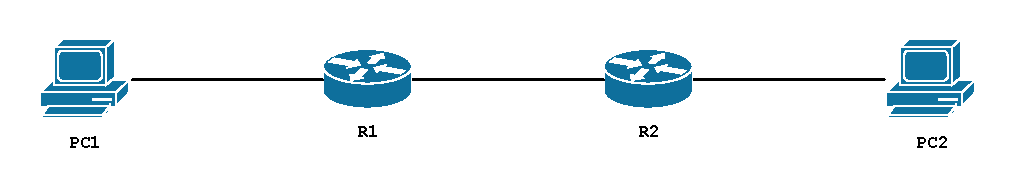
\includegraphics[width=\linewidth]{topology}
	\caption{Η τοπολογία του δικτύου προς υλοποίηση}\label{fig:topology}
\end{figure}

\paragraph{Σενάριο:} Υποθέστε ότι σας δίνεται η ομάδα διευθύνσεων \textbf{\texttt{10.8.0.0/16},} η οποία πρέπει να χωριστεί σε \textbf{4} ισομεγέθη υποδίκτυα και να ανατεθεί στα αντίστοιχα υποδίκτυα της τοπολογίας του σχήματος~\ref{fig:topology}.

\paragraph{Βήμα 1:} Αρχικά, θα πρέπει να καθοριστεί το μέγεθος του κάθε υποδικτύου. Συμπληρώστε στο πεδίο που ακολουθεί το μήκος προθέματος του κάθε δικτύου, λαμβάνοντας υπόψιν ότι χωρίζετε το αρχικό δίκτυο σε 4 υποδίκτυα ίδιου μεγέθους.\\[0.25cm]
Νέο μήκος προθέματος: \textField[\BC{0 0 1}\BG{0.98 0.92 0.73}]{8}{1.5cm}{0.75cm}

\paragraph{Βήμα 2:} Ορίστε τα προκύπτοντα υποδίκτυα με μορφή CIDR (πχ \texttt{192.168.1.0/24}), συμπληρώνοντας την παρακάτω φόρμα:

\begin{table}[ht]
	\centering
	\begin{tabular}{ll}
		Δίκτυο \#0 & \textField{9}{3cm}{0.65cm} \\[0.25cm]
		Δίκτυο \#1 & \textField{10}{3cm}{0.65cm} \\[0.25cm]
		Δίκτυο \#2 & \textField{11}{3cm}{0.65cm} \\[0.25cm]
		Δίκτυο \#3 & \textField{12}{3cm}{0.65cm} \\
	\end{tabular}
\end{table}

\paragraph{Βήμα 3:} Συμπληρώστε τον πίνακα \ref{tab:scenario1}, αναθέτοντας διευθύνσεις IP στους δρομολογητές, στους υπολογιστές και τις SVI των μεταγωγέων με βάση την υποδικτύωση FLSM που εφαρμόσατε νωρίτερα. Κατά τη συνήθη πρακτική, αναθέστε στους δρομολογητές/πύλες των υποδικτύων την πρώτη ωφέλιμη IP. Για τους ξενιστές ακολουθήστε τα εξής:
\begin{itemize}\setlength{\itemsep}{-0.075cm}
	\item S1, S2: Τελευταία ωφέλιμη IP του δικτύου στο οποίο ανήκουν
	\item PC1: $7^\text{η}$ ωφέλιμη IP
	\item PC2: $84^\text{η}$ ωφέλιμη IP
\end{itemize}

\begin{table}[ht]
	\centering\renewcommand\arraystretch{1.5}
	\begin{tabular}{lllll}
		\FormatFirstRow
		\textbf{Συσκευή} & \textbf{Διεπαφή} & \textbf{Διεύθυνση IP}				& \textbf{Μάσκα υποδικτύου}		& \textbf{Προεπιλεγμένη πύλη}\\
						 & \ip{Gi0/0}		& \textField{13}{3cm}{0.5cm}		& \textField{22}{3cm}{0.5cm} 	& \\
						 & \ip{Gi0/1}		& \textField{14}{3cm}{0.5cm}		& \textField{23}{3cm}{0.5cm}	& \\
\multirow{-3}{*}{R1}	 & \ip{Gi0/2}		& \textField{15}{3cm}{0.5cm}	 	& \textField{24}{3cm}{0.5cm} 	& \multirow{-3}{*}{\textField{31}{3cm}{0.5cm}} \\
\rowcolor{lightgray}	 & \ip{G0/0}		& \textField{16}{3cm}{0.5cm}		& \textField{25}{3cm}{0.5cm} 	& \\
\rowcolor{lightgray}
\multirow{-2}{*}{R2}	 & \ip{G0/1}		& \textField{17}{3cm}{0.5cm}	 	& \textField{26}{3cm}{0.5cm}	& \multirow{-2}{*}{\textField{32}{3cm}{0.5cm}}\\
	S1  				 & SVI	  			& \textField{18}{3cm}{0.5cm}		& \textField{27}{3cm}{0.5cm} 	& \textField{33}{3cm}{0.5cm}\\
\rowcolor{lightgray}
	S2  				 & SVI	  			& \textField{19}{3cm}{0.5cm}		& \textField{28}{3cm}{0.5cm} 	& \textField{34}{3cm}{0.5cm}\\	
	PC1  				 & NIC	  			& \textField{20}{3cm}{0.5cm}		& \textField{29}{3cm}{0.5cm} 	& \textField{35}{3cm}{0.5cm}\\
\rowcolor{lightgray}
	PC2					 & NIC	  			& \textField{21}{3cm}{0.5cm}		& \textField{30}{3cm}{0.5cm}	& \textField{36}{3cm}{0.5cm}\\
	\end{tabular}
	\caption{Σχήμα διευθυνσιοδότησης για το σενάριο FLSM.}\label{tab:scenario1}
\end{table}

\paragraph{Βήμα 4:} Εφαρμόστε τα δεδομένα του πίνακα \ref{tab:scenario1} στις δικτυακές συσκευές και τους υπολογιστές. Πρόσθετα, ορίστε προεπιλεγμένη πύλη δικτύου για τους δυο δρομολογητές, ώστε να καταστεί εφικτή η επικοινωνία των απομακρυσμένων δικτύων.

\paragraph{Βήμα 5:} Δοκιμάστε τη σύνδεση του PC1 με τον PC2 χρησιμοποιώντας την εντολή \texttt{tracert}.

\begin{assignmentbox}
		 Αποθηκεύστε σε εξωτερικό αρχείο και παραδώστε τις τρέχουσες ρυθμίσεις των δρομολογητών R1 και R2
		 Παραδώστε ένα στιγμιότυπο οθόνης που δείχνε την επιτυχή εκτέλεση της εντολής \texttt{tracert}.
\end{assignmentbox}

\newpage

\section{Σενάριο: Υποδικτύωση VLSM}

Τροποποιήστε την τοπολογία του σχήματος \ref{fig:topology}, μετακινώντας τον S2 στη διεπαφή \ip{G0/2} του R2. H νέα τοπολογία που προκύπτει απεικονίζεται στο σχήμα \ref{fig:topology2}.

\begin{figure}[ht]
	\centering
	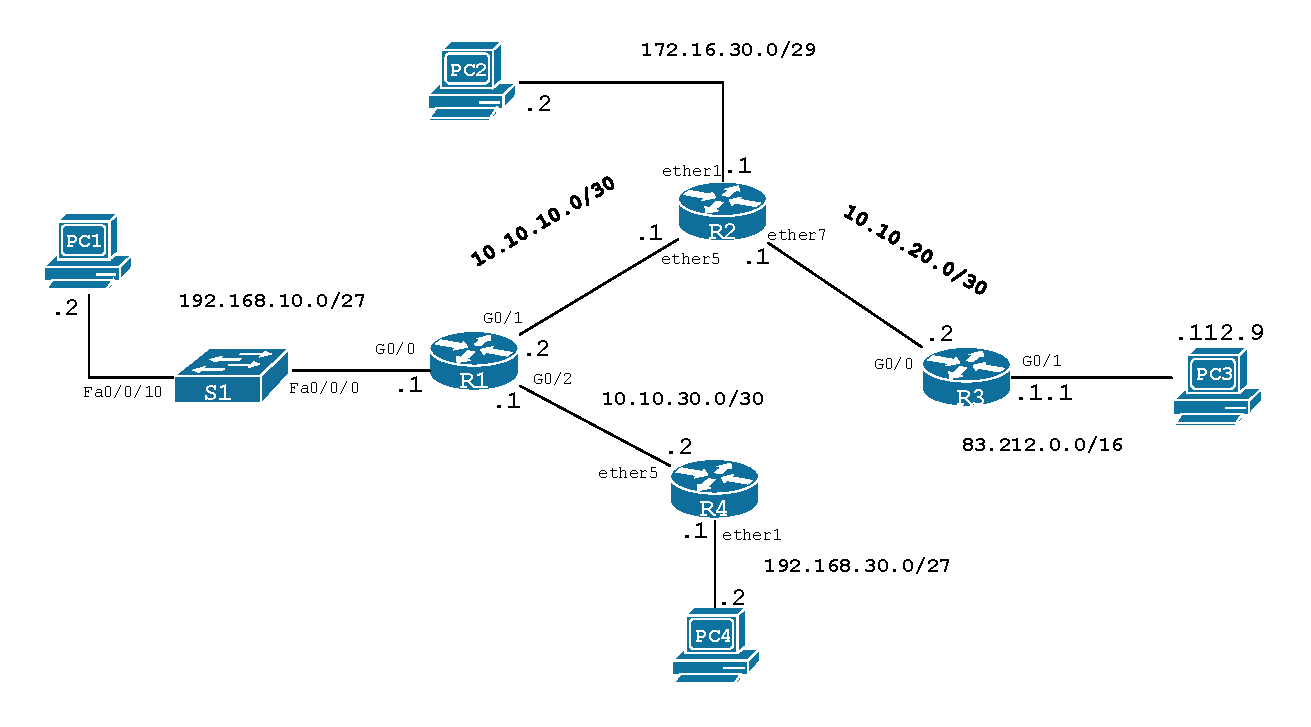
\includegraphics[width=0.85\linewidth]{topology2}
	\caption{Η νέα τοπολογία για το σενάριο VLSM}\label{fig:topology2}
\end{figure}

\textbf{Σενάριο:} Υποθέστε ότι σας ανατίθεται από την αρμόδια υπηρεσία ανάθεσης διευθύνσεων της περιοχής σας (Regional Internet Registry - RIR) η ομάδα διευθύνσεων \textbf{\texttt{135.56.0.0/16}}, η οποία πρέπει να κατανεμηθεί στα δίκτυα της τοπολογίας του σχήματος \ref{fig:topology2}. Κάθε επιμέρους δίκτυο έχει διαφορετικές ανάγκες σε πλήθος ξενιστών, συνεπώς, τα επιμέρους υποδίκτυα που θα προκύψουν από την ομάδα \ip{135.56.0.0/16} πρέπει να έχουν διαφορετικό μέγεθος. Οι απαιτήσεις καταγράφονται στον πίνακα \ref{tab:req}.

\begin{table}[ht]\renewcommand\arraystretch{1.5}
	\centering\rowcolors{2}{lightgray}{white}
	\begin{tabular}{ccm{3.5cm}m{4cm}}
		\FormatFirstRow \textbf{Υποδίκτυο} & \textbf{Ελάχιστο πλήθος ωφέλιμων IP} & \textbf{Μάσκα υποδικτύου}	&\textbf{Διεύθυνση δικτύου σε μορφή CIDR}\\
		Α 								   & 760 						 		  &\textField{37}{3cm}{0.5cm}	&\textField{71}{3cm}{0.5cm}\\
		Β 					   			   & 256 						 		  &\textField{0}{3cm}{0.5cm}  	&\textField{41}{3cm}{0.5cm}\\
		Γ 					   			   & 1700						 		  &\textField{38}{3cm}{0.5cm} 	&\textField{42}{3cm}{0.5cm}\\
		Δ 					   			   & 160 						  		  &\textField{39}{3cm}{0.5cm}  	&\textField{43}{3cm}{0.5cm}\\
		Ε 					   			   & 2 						 	 		  &\textField{40}{3cm}{0.5cm}  	&\textField{44}{3cm}{0.5cm}
	\end{tabular}
	\caption{Οι απαιτήσεις για κάθε υποδίκτυο και οι αντίστοιχες μάσκες υποδικτύου.}\label{tab:req}
\end{table}


\paragraph{Βήμα 1:} Αρχικά, θα πρέπει να καθοριστούν οι μάσκες των υποδικτύων που καλύπτουν τις απαιτήσεις. Συμπληρώστε την τρίτη στήλη του πίνακα \ref{tab:req} με τις μάσκες των υποδικτύων σε δεκαδική μορφή, οι οποίες εκπληρούν τις ελάχιστες απαιτήσεις σε πλήθος ωφέλιμων IP.

\paragraph{Βήμα 2:} Έχοντας ορίσει τις μάσκες μπορείτε να προσδιορίσετε πλήρως τις διευθύνσεις δικτύου των νέων υποδικτύων. Η τεχνική VLSM απαιτεί να ξεκινήσετε από το μεγαλύτερο και να καταλήξετε στο μικρότερο υποδίκτυο, συνεπώς, ξεκινήστε την τεχνική VLSM από το μεγαλύτερο προς το μικρότερο υποδίκτυο και συμπληρώστε την τελευταία στήλη του πίνακα \ref{tab:req}.\vspace{-0.25cm}

\paragraph{Βήμα 3:} Συμπληρώστε τον πίνακα \ref{tab:scenario2}, αναθέτοντας διευθύνσεις IP στους δρομολογητές, τους υπολογιστές και τις SVI των μεταγωγέων με βάση την υποδικτύωση VSLM που εφαρμόσατε. Κατά τη συνήθη πρακτική, αναθέστε στους δρομολογητές την πρώτη ή τη δεύτερη (αν δεν είναι διαθέσιμη η πρώτη) ωφέλιμη IP. Για τους ξενιστές ακολουθήστε τα εξής:
\begin{itemize}
	\setlength\itemsep{-0.75em}
	\item S1, S2: Τελευταία ωφέλιμη IP του δικτύου στο οποίο ανήκουν.
	\item PC1: $14^\text{η}$ ωφέλιμη IP.
	\item PC2: $35^\text{η}$ ωφέλιμη IP.
\end{itemize}

\begin{table}[ht]
	\centering\renewcommand\arraystretch{1.5}
	\begin{tabular}{lllll}
		\FormatFirstRow
		\textbf{Συσκευή} & \textbf{Διεπαφή} & \textbf{Διεύθυνση IP}				& \textbf{Μάσκα υποδικτύου}			& \textbf{Προεπιλεγμένη πύλη}\\
					 & \ip{Gi0/0}		& \textField{45}{3cm}{0.5cm}		& \textField{55}{3cm}{0.5cm}		& \\
					 & \ip{Gi0/1}		& \textField{46}{3cm}{0.5cm}		& \textField{56}{3cm}{0.5cm} 		& \\
\multirow{-3}{*}{R1}	 & \ip{Gi0/2}		& \textField{47}{3cm}{0.5cm}	 	& \textField{57}{3cm}{0.5cm} 		& \multirow{-3}{*}{\textField{65}{3cm}{0.5cm}} \\
\rowcolor{lightgray}	 & \ip{G0/0}		& \textField{48}{3cm}{0.5cm}		& \textField{58}{3cm}{0.5cm} 		& \\
\rowcolor{lightgray}	 & \ip{G0/1}		& \textField{49}{3cm}{0.5cm}		& \textField{59}{3cm}{0.5cm}		& \\
\rowcolor{lightgray}
\multirow{-3}{*}{R2}	 & \ip{G0/2}		& \textField{50}{3cm}{0.5cm}	 	& \textField{60}{3cm}{0.5cm}		& \multirow{-3}{*}{\textField{66}{3cm}{0.5cm}}\\
			S1  		 & SVI	  			& \textField{51}{3cm}{0.5cm}		& \textField{61}{3cm}{0.5cm} 		& \textField{67}{3cm}{0.5cm}\\
\rowcolor{lightgray}S2  	 & SVI	  			& \textField{52}{3cm}{0.5cm}		& \textField{62}{3cm}{0.5cm} 		& \textField{68}{3cm}{0.5cm}\\	
			PC1  		 & NIC	  			& \textField{53}{3cm}{0.5cm}		& \textField{63}{3cm}{0.5cm} 		& \textField{69}{3cm}{0.5cm}\\
\rowcolor{lightgray}PC2		 & NIC	  			& \textField{54}{3cm}{0.5cm}		& \textField{64}{3cm}{0.5cm} 		& \textField{70}{3cm}{0.5cm}\\
	\end{tabular}
	\caption{Σχήμα διευθυνσιοδότησης για το σενάριο VLSM.}\label{tab:scenario2}
\end{table}

\paragraph{Βήμα 4:} Εφαρμόστε τα δεδομένα του πίνακα \ref{tab:scenario2} στις συσκευές Cisco και τους υπολογιστές. Πρόσθετα, ορίστε προεπιλεγμένη πύλη δικτύου για τους δυο δρομολογητές, ώστε να καταστεί εφικτή η επικοινωνία των απομακρυσμένων δικτύων.

\paragraph{Βήμα 5:} Δοκιμάστε τη σύνδεση του PC1 με τον PC2 χρησιμοποιώντας την εντολή \texttt{tracert}.

\begin{assignmentbox}
	Αποθηκεύστε σε εξωτερικό αρχείο και παραδώστε τις τρέχουσες ρυθμίσεις των δρομολογητών R1 και R2.
\end{assignmentbox}

\begin{assignmentbox}
	Παραδώστε ένα στιγμιότυπο οθόνης που δείχνει την επιτυχή εκτέλεση της εντολής \texttt{tracert}.
\end{assignmentbox}

\end{document}